\chapter{TEMPLATE E STRATEGY}
Sono due pattern \underline{comportamentali}, descrivono come classi e oggetti interagiscono e si distribuiscono le responsabilità.

\section{Template Method}
Definisce, in unico punto, lo scheletro di un algoritmo e delega alcuni passi, quelli che possono variare, alle sottoclassi che avranno il compito di ridefinirli senza
modificare la struttura dell'algoritmo stesso.

Prendiamo come esempio un framework che fornisce le classi Application e Document responsabili, rspettivamente, di aprire un documento e salvarlo e di rappresentare 
le informazioni una volta che il documento è in memoria.

Application, intesa come classe astratta, definirà l’algoritmo per aprire e leggere un documento in un metodo openDocument() che chiamerà al suo interno altri metodi 
di utilità, astratti, che saranno implementati dalle sottoclassi.

Il metodo openDocument() è il nostro templateMethod.
\begin{lstlisting}
public abstract class Application {
    private List<Document> docs;
    // costruttore...
    
    public final void openDocument(String path) {
        if (!canOpenDocument(path)) {
            // gestisce l'errore
        }
        Document doc = doCreateDocument(path);
        docs.add(doc);
        aboutToOpenDoc(doc);
        doc.open();
        doc.doRead();
    }

    protected abstract void aboutToOpenDoc(Document doc);
    protected abstract Document doCreateDocument(String path);
    protected abstract boolean canOpenDocument(String path);
}
\end{lstlisting}

e chi intenderà utilizzare il nostro framework dovrà estendere le classi Application e Document, ridefinendo i metodi astratti.

Il templateMethod porta all'\textit{hollywood principle}, ovvero sono le classi parent a chiamare i metodi delle sottoclassi e non l'inverso. 

\medskip
\textbf{N.B.} Sapendo che il templateMethod non cambiarà mai, allora potremmo renderlo final.

\subsection{Struttura e partecipanti}

\begin{figure}[H]
    \centering
    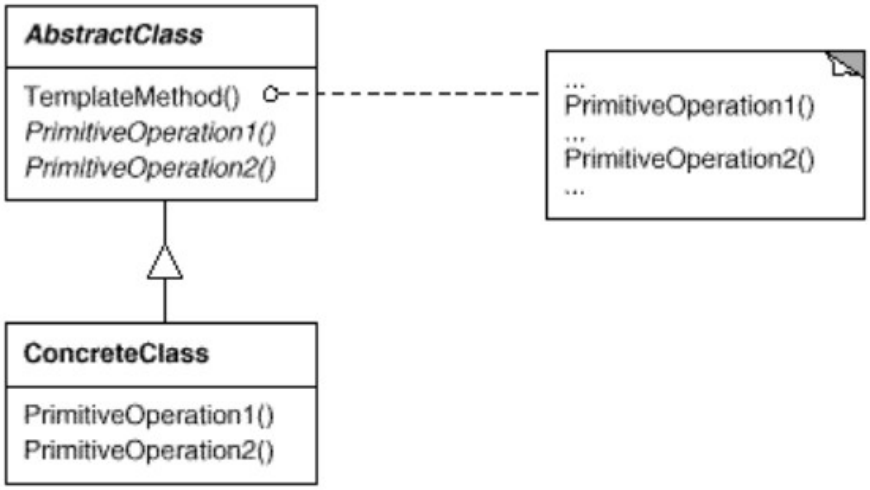
\includegraphics[width=0.4\linewidth]{../../immagini/templateMethod_Strategy/struttura_templateMethod}    
\end{figure}

\textbf{AbstractClass} 

\begin{itemize}
    \item \textit{definisce} le operazioni astratte che rappresentano i passi di un algoritmo;
    \item \textit{Implementa} il template method (l’algoritmo) che, a sua volta, chiama le operazioni astratte.
\end{itemize}

\textbf{ConcreteClass} che implementa le operazioni astratte.

\section{Strategy}

Definisce una famiglia di algoritmi, li incapsula, li rende intercambiabili e ne nasconde le informazioni interne cosicchè una classe può avere diversi comportamenti 
a seconda di qualche condizione.
\smallskip

Prendiamo ad esempio una classe Shop che può applicare più tipologie di sconti ad esempio percentuale, assoluto o nessuno sconto.

Prima di applicare lo Strategy saremo in una condizione di questo tipo
\begin{lstlisting}
public class Shop {
    private DiscountType discountType;
        public Shop(DiscountType discountType) {
        this.discountType = discountType;
    }

    public void setDiscountType(DiscountType discountType) {
        this.discountType = discountType;
    }

    public int getTotal(int originalPrice) {
        switch (discountType) {
        case NO_DISCOUNT:
            return originalPrice;
        case ABSOLUTE_DISCOUNT:
            // sottrae un valore predefinito
            // (predefinito dove?)
            return ...;
        case PERCENTAGE_DISCOUNT:
            // applica uno sconto su percentuale
            // (quale percentuale?)
            return ...;
        }
        return ...;
    }
}
\end{lstlisting}

dove il tipo di sconto può essere modificato a runtime (good) ma i dettagli interni di ogni tipo di sconto devono essere specificati nello Shop (no good) e, se 
in futuro dovessi aggiungere un nuovo tipo di sconto, dovrei mettere mano alla classe Shop aggiungengo un nuovo ramo all'if-else, anche se non dovrebbe essere di sua 
compentenza.

Con lo Strategy avremo 
\begin{lstlisting}
public class Shop {

private DiscountStrategy discountStrategy;
    public Shop(DiscountStrategy discountStrategy) {
        this.discountStrategy = discountStrategy;
    }

    public void setDiscountStrategy(DiscountStrategy discountStrategy) {
        this.discountStrategy = discountStrategy
    }

    public int getTotal(int originalPrice) {
        return discountStrategy.applyDiscount(originalPrice);
    }
}
\end{lstlisting}

dove il tipo di sconto può essere modificato a runtime (good) e dettagli interni di ogni tipo di sconto non riguardano Shop (good).

DiscountStrategy è la nostra interfaccia che mette a disposizione il metodo astratto, applyDiscount(int) che sarà gestito in maniera differente in base alla tipologia
di sconto che vogliamo applicare, ad esempio
\newpage
\begin{multicols}{2}
\begin{lstlisting}
    public interface DiscountStrategy {
        int applyDiscount(int originalPrice);
    }
\end{lstlisting}
\columnbreak
\begin{lstlisting}
    public class NoDiscountStrategy implements DiscountStrategy {
        @Override
        public int applyDiscount(int originalPrice) {
            return originalPrice;
        }
    }
\end{lstlisting}
\end{multicols}

\begin{multicols}{2}
\begin{lstlisting}
    public class AbsoluteDiscountStrategy implements DiscountStrategy {
    private int discount;
    
    public AbsoluteDiscountStrategy(int discount) {
        this.discount = discount;
    }

    @Override
    public int applyDiscount(int originalPrice) {
        return originalPrice - discount;
    }
}    
\end{lstlisting}
\columnbreak
\begin{lstlisting}
    public class PercentageDiscountStrategy implements DiscountStrategy {
    private int percentage;
    
    public PercentageDiscountStrategy(int percentage) {
        this.percentage = percentage;
    }

    @Override
    public int applyDiscount(int originalPrice) {
        return originalPrice - (originalPrice * percentage / 100);
    }
}
\end{lstlisting}
\end{multicols}

\subsection{Conseguenza}

I Client devono essere consapevoli che esistono diverse strategie (cioè diverse implementazioni di una strategia), infatti hanno un riferimento allo Strategy.

\subsection{Struttura e partecipanti}

\begin{figure}[H]
    \centering   
    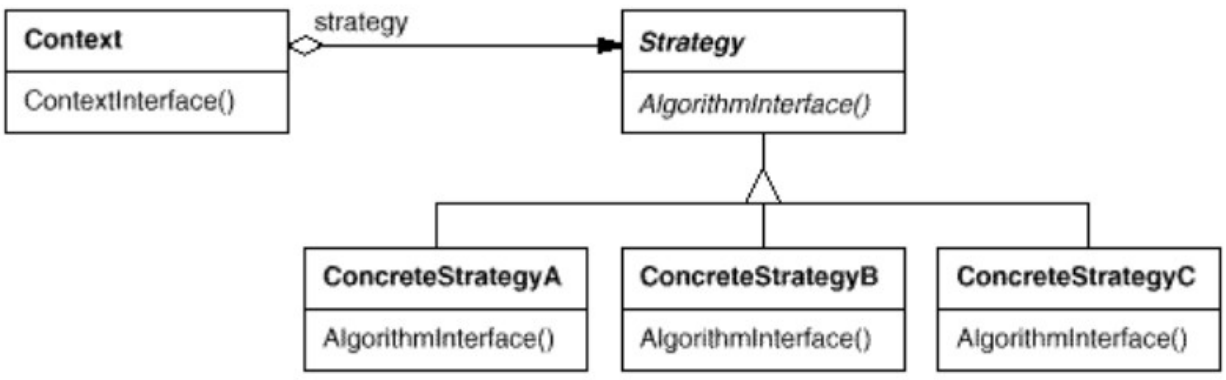
\includegraphics[width=0.5\linewidth]{../../immagini/templateMethod_Strategy/struttura_strategy}    
\end{figure}

\textbf{Strategy} dichiara l’interfaccia comune a tutti gli algoritmi supportati;

\textbf{ConcreteStrategy} implementa l’interfaccia Strategy e l’algoritmo;

\textbf{Context} usa uno Strategy quando ha bisogno dell’algoritmo che, a runtime, sarà effettivamente implementato da un ConcreteStrategy.

Context ha un riferimento a Strategy che sarà configurato assegnandogli un ConcreteStrategy passandolo al costruttore o tramite un setter, inoltre può definire a sua 
volta un’interfaccia per permettere a uno Strategy di accedere al suo stato.

\subsection{Differenza con il templateMethod}

Sembra simile al templateMethod, invece è completamente l'opposto, col templateMethod l'\textit{implementazione dell'algoritmo è fissa}, cambia solamente 
l'implementazione di alcuni suoi passi, mentre nello strategy è \textit{fisso il problema che intende risovere} l'algoritmo ma il come deve essere risolto viene 
implementato dalle sottoclassi. 
\smallskip

Prendiamo come esempio l'ordinamento

\begin{itemize}
    \item con il templateMethod avremo il Bubblesort come algoritmo fisso, dove al suo interno potranno \textbf{cambiare alcuni suoi passi}, quindi le sottoclassi
    estenderanno la classe Bubblesort ed implementeranno i suoi passi astratti;
    \item con lo Strartegy, si definisce un'interfaccia per l'ordinamento dove l'\textbf{algoritmo cambia}, a seconda del tipo di ordinamento,  
    (SelectionSort, InsertionSort, Bubblesort, ecc\dots..), quindi le sottoclasse implementeranno l'ordinamento desiderato e ridefiniranno l'algoritmo a proprio 
    piacimento.
\end{itemize}

Template Method sfrutta l’inheritance e l’overriding (meccanismo statico), mentre lo Strategy sfrutta l’object composition e delegation (meccanismo dinamico), 
infatti l’implementazione di strategy può essere anche modificata a runtime, ad esempio tramite il setter.

\subsection{Strategy e classi anonime}

Si può creare una classe di utilità che crea le strategy con classi anonime
\begin{lstlisting}
public class DiscountStrategies {

    //costruttore privato

    public static DiscountStrategy noDiscount() {
        return new DiscountStrategy() {
            @Override
            public int applyDiscount(int originalPrice) {
                return originalPrice;
            }
        };
    }

    public static DiscountStrategy absoluteDiscount(int discount) {
        return new DiscountStrategy() {
            @Override
            public int applyDiscount(int originalPrice) {
                return originalPrice - discount;
            }
        };
    }

    public static DiscountStrategy percentageDiscount(int percentage) {
        return new DiscountStrategy() {
            @Override
            public int applyDiscount(int originalPrice) {
                return originalPrice - (originalPrice * percentage / 100);
            }
        };
    }
}
\end{lstlisting}

\subsection{Strategy e lambda}

L’interfaccia Strategy di solito ha un singolo metodo astratto, quindi siamo in contesto lambda.
\begin{lstlisting}
public class DiscountStrategies {
    public static DiscountStrategy noDiscount() {
        return originalPrice -> originalPrice;
    }

    public static DiscountStrategy absoluteDiscount(int discount) {
        return originalPrice -> originalPrice - discount;
    }

    public static DiscountStrategy percentageDiscount(int percentage) {
        return originalPrice -> originalPrice - (originalPrice * percentage / 100);
    }
}
\end{lstlisting}